
% ===============================================
% MATH 34: Multivariable calculus           Spring 2019
% hw_template.tex
% ===============================================

% -------------------------------------------------------------------------
% You can ignore this preamble. Go on
% down to the section that says "START HERE" 
% -------------------------------------------------------------------------

\documentclass{article}

\usepackage[margin=1.5in]{geometry} % Please keep the margins at 1.5 so that there is space for grader comments.
\usepackage{amsmath,amsthm,amssymb,hyperref}
\usepackage{mathtools}
\usepackage{graphicx}
\usepackage{float}
\usepackage{listings}
\usepackage{xparse}
\usepackage{xcolor}
\usepackage{verbatim}

\newcommand{\R}{\mathbf{R}}  
\newcommand{\Z}{\mathbf{Z}}
\newcommand{\N}{\mathbf{N}}
\newcommand{\Q}{\mathbf{Q}}
\newcommand{\C}{\mathbf{C}}
\newcommand{\Log}{\text{Log}}
\newcommand{\Arg}{\text{Arg}}
\newcommand{\Real}{\text{Re}}
\newcommand{\Imag}{\text{Im}}
\newcommand{\ddz}{\frac{d}{dz}}

\newenvironment{theorem}[2][Theorem]{\begin{trivlist}
\item[\hskip \labelsep {\bfseries #1}\hskip \labelsep {\bfseries #2.}]}{\end{trivlist}}
\newenvironment{lemma}[2][Lemma]{\begin{trivlist}
\item[\hskip \labelsep {\bfseries #1}\hskip \labelsep {\bfseries #2.}]}{\end{trivlist}}
\newenvironment{claim}[2][Claim]{\begin{trivlist}
\item[\hskip \labelsep {\bfseries #1}\hskip \labelsep {\bfseries #2.}]}{\end{trivlist}}
\newenvironment{problem}[2][Problem]{\begin{trivlist}
\item[\hskip \labelsep {\bfseries #1}\hskip \labelsep {\bfseries #2.}]}{\end{trivlist}}
\newenvironment{proposition}[2][Proposition]{\begin{trivlist}
\item[\hskip \labelsep {\bfseries #1}\hskip \labelsep {\bfseries #2.}]}{\end{trivlist}}
\newenvironment{corollary}[2][Corollary]{\begin{trivlist}
\item[\hskip \labelsep {\bfseries #1}\hskip \labelsep {\bfseries #2.}]}{\end{trivlist}}

\DeclarePairedDelimiter\abs{\lvert}{\rvert}

\newenvironment{solution}{\begin{proof}[Solution]}{\end{proof}}

\makeatletter
\newcommand{\skipitems}[1]{%
	\addtocounter{\@enumctr}{#1}%
}
\makeatother

\NewDocumentCommand{\codeword}{v}{%
\texttt{\textcolor{blue}{#1}}%
}


\begin{document}

\large % please keep the text at this size for ease of reading.

% ------------------------------------------ %
%                 START HERE             %
% ------------------------------------------ %

{\Large Page 1 % Replace with appropriate page number 
\hfill  MTH483, Complex Variables, HW7}

\begin{center}
{\Large Wyatt Whiting}
\end{center}
\vspace{0.05in}

% -----------------------------------------------------
% The "enumerate" environment allows for automatic problem numbering.
% To make the number for the next problem, type " \item ". 
% To make sub-problems such as (a), (b), etc., use an "enumerate" within an "enumerate."
% -----------------------------------------------------
\begin{enumerate}
	\item Find the radius of convergence and the region of convergence of the following power series:
	\begin{enumerate}
		\item $\sum_{n=1}^{\infty}\frac{(2z)^n}{1+3^n}$
		
		Applying the ratio test:
		
		\[\lim_{n \to\infty}\abs*{\frac{(2z)^{n+1}}{1+3^{n+1}} \frac{1+3^n}{(2z)^n}} =\lim_{n \to\infty}\abs*{\frac{2z(1+3^n)}{1+3^{n+1}}}=\frac{2|z|}{3} \]
		
		We demand that $\frac{2|z|}{3}<1$, so then $|z|<\frac{3}{2}$, so the radius of convergence is $\frac{3}{2}$. We can then conclude that the region of convergence is $D_{3/2}(0)$
		
		\item $\sum_{n=1}^{\infty}\frac{z^n}{(\sqrt{3}+i)^n} = \sum_{n=1}^{\infty}(\frac{z}{\sqrt{3}+i})^n$
		
		The form of the summand make applying the root test quite easy:
		
		\[\lim_{n \to\infty}\sqrt[n]{\left(\frac{z}{\sqrt{3}+i}\right)^n} =\frac{z}{\sqrt{3}+i}\]
		
		To converge, we demand $\frac{|z|}{|\sqrt{3}+i|}<1 \implies \frac{|z|}{2}<1\implies |z|<2$, so the radius of convergence is $2$. Then the region of convergence is $D_4(0)$.
	\end{enumerate}
	
	\item Find three different Laurent series representations (about 0) for the function 
	\[f(z)=\frac{3}{-z^2+z+2}=\frac{1}{z+1}-\frac{1}{z-2} \]
	
	We can see that the function has two singularities at $z=-1$ and $z=2$. These split the plane into three regions with varying radius. Let's begin with the region $|z|<1$.
	
	The function is holomorphic on $D_1(0)$ since it contains no singularities. Then our Laurent series ends up being a regular Taylor series given by 
	
	\[ f(z)=\frac{3}{-z^2+z+2}=\frac{1}{1+z}+\frac{1}{2-z}=\sum_{k=0}^{\infty}(-z)^k+\ \sum_{k=0}^{\infty}\frac{z^k}{2^{k+1}} \]
	
	\[=\sum_{k=0}^{\infty}(-z)^k+\frac{z^k}{2^{k+1}}, \]
	
	which holds when $|z|<1$.
	
	Now we focus on the annulus $1<|z|<2$. We can manipulate the terms as follows:
	
	\[\frac{1}{1+z}=\frac{1}{z}\frac{1}{\frac{1}{z}+1}=\frac{1}{z}\sum_{k=0}^{\infty}\frac{(-1)^k}{z^k}=\sum_{k=0}^{\infty}\frac{(-1)^k}{z^{k+1}}, \]
	
	which converges when $|z|>1$. We can also expand the other term, giving
	
	\[\frac{1}{2-z}=\sum_{k=0}^{\infty}\frac{z^k}{2^{k+1}}, \]
	
	 which holds for $|z|<2$. Combining these gives 
	 
	 \[f(z)=\frac{1}{z+1}+\frac{1}{2-z}=\sum_{k=0}^{\infty}\frac{(-1)^k}{z^{k+1}}+\sum_{k=0}^{\infty}\frac{z^k}{2^{k+1}}=\sum_{k=0}^{\infty}\frac{(-1)^k}{z^{k+1}}+\frac{z^k}{2^{k+1}}, \]
	 
	 which holds for $1<|z|<2$. 
	 
	 Finally, let's examine the case $|z|>2$. We can recycle the manipulation of $\frac{1}{1+z}$ from above since its valid for $|z|>1$. For the other term, we have
	 
	 \[\frac{1}{2-z}=\frac{1}{z}\frac{1}{\frac{2}{z}-1} = -\frac{1}{z}\frac{1}{1-\frac{2}{z}}=-\frac{1}{z}\sum_{k=0}^{\infty}\frac{2^k}{z^k}=-\sum_{k=0}^{\infty}\frac{2^k}{z^{k+1}}, \]
	 
	 which holds for $|z|>2$. Combining the two series gives
	 
	 \[f(z)= \frac{1}{z+1}+\frac{1}{2-z}=\sum_{k=0}^{\infty}\frac{(-1)^k}{z^{k+1}}-\sum_{k=0}^{\infty}\frac{2^k}{z^{k+1}} \]
	 
	 \[=\sum_{k=0}^{\infty}\frac{(-1)^k-2^k}{z^{k+1}}, \]
	 
	 which holds for all $|z|>2$. Thus, these are three different Laurent series for $f(z)=\frac{3}{-z^2+z+2}$.
	
	\item 
	\begin{enumerate}
		\item Sketch $\gamma$.
		
		\codeword{ p[s_] := ParametricPlot[{3 Cos[t] Cos[3 t], 3 Sin[t] Cos[3 t]}, {t, 0, s}, PlotRange -> {{-3, 3}, {-3, 3}}] }
    
    	\codeword{Manipulate[p[t], {t, 0.1, 2 Pi}]}
    	
    	This code allows me to use the slider to watch what happens to the graph of $\gamma$ as the range of t is varied. It's from this that we see that each lobe has positive orientation as t is increasing.
    
   	 	\begin{figure}[H]
   	 	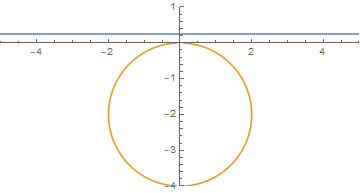
\includegraphics[scale=0.8]{image2.png}
   	 	\end{figure}
    
    	We can see that the figure completes an entire loop and touches its endpoint when $t=\pi$. Thus, since $t\in[0,2\pi]$, $\gamma$ traces itself twice.
    	
    	\item Compute the exact value of $\int_{\gamma}f(z)\ dz$
    	
    	In order the compute this integral, we will split up $\gamma$ into its three lobes and evaluate them separately. Let the rightmost lobe be $\gamma_1$ and working counterclockwise, the next two lobes be $\gamma_2$ and $\gamma_3$. By watching the manipulation of $\gamma$ with Mathematica, we can each region is positively oriented.
    	
    	Let's begin with $\gamma_1$. We can see that $\gamma_1$ encloses the point $a=1$. We can then apply Cauchy's integral formula by rearranging the integrand as follows:
    	
    	\[\int_{\gamma_1}f(z)\ dz = \int_{\gamma_1}\frac{1}{(z^2+2z+2)(z-1)}\ dz = \int_{\gamma_1}\frac{\frac{1}{(z^2+2z+2)}}{z-1}\ dz \]
    \[=2\pi i \frac{1}{1+2+2}=\frac{2\pi i}{5} \]
    
    Now let's examine $\gamma_2$ in a simliar fashion. We can see the point $a=-1+i$ is contained within $\gamma_2$, which is also a root of the second degree polynomial. We can then rearrange the integral as follows:
    
    \[\int_{\gamma_2}\frac{1}{(z^2+2z+2)(z-1)}\ dz = \int_{\gamma_2}\frac{\frac{1}{(z+1+i)(z-1)}}{z+1-i}\ dz \]
    \[ = 2\pi i\frac{1}{((-1+i)-1)((-1+i)+1+i)} = 2\pi i \frac{1}{(-2+i)(2i)} \]
    \[ =\frac{2\pi i}{-2-4i}=\frac{\pi i}{-1-2i}\] 
    
    Finally, let's evaluate $\gamma_3$ in a similar fashion. I omit explanation for obvious reasons.
    
    \[\int_{\gamma_3}\frac{1}{(z^2+2z+2)(z-1)\  }\ dz = \int_{\gamma_3}\frac{\frac{1}{(z-1)(z+1-i)}}{z+1+i} \]
    \[=2\pi i\frac{1}{((-1-i)-1)((-1-i)+1-i)} =2\pi i \frac{1}{(-2-i)(-2i)}\]
    \[=\frac{2\pi i}{-2+4i} =\frac{\pi i}{-1+2i}\]
    
    Now we add the integrals together:
    
    \[\int_{\gamma}f(z)\ dz= \int_{\gamma_1}f(z)\ dz + \int_{\gamma_2}f(z)\ dz + \int_{\gamma_3}f(z)\ dz \]
    \[= \frac{2\pi i}{5}+\frac{\pi i}{-1-2i}+\frac{\pi i}{-1+2i} = 0\]
	\end{enumerate}
	
	\item 
	\begin{enumerate}
		\item Sketch $\gamma$.
		
		\codeword{p[s_] := ParametricPlot[{Sin[t] + Sin[2 t], Cos[t] + Cos[5 t]}, {t, 0, s}, PlotRange -> {{-2.5, 2.5}, {-2.5, 2.5}}]}
		
		\codeword{ Manipulate[p[s], {s, 0.1, Pi}] }
		
		Similar to the previous code, this enters $\gamma$ as a parametrized curve and then allows me to view how $\gamma$ is traced as t varies from 0 to $\pi$.
		
		\begin{figure}[H]
		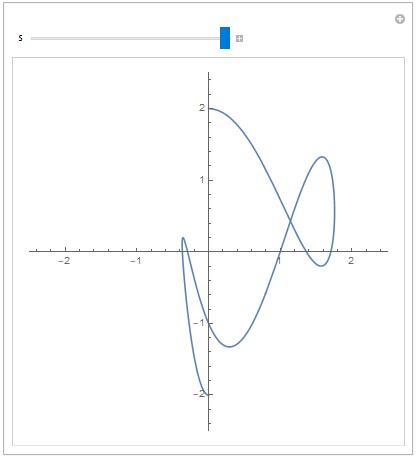
\includegraphics[scale=0.8]{image3.png}
		\end{figure}
		
		We can see that $\gamma$ takes a very strange path. It is not "nice" as in the previous problem, which makes integration over $\gamma$ a somewhat more formidable task.
		
		\item Find a Laurent series representation of $f(z)$ about 0.
		
		Luckily for us, the form of this function makes finding a proper Laurent series exceedingly easy. Observe:
		
		\[f(z)=\frac{e^z}{z^3}=z^{-3}e^z \]
		
		We already know a series expansion for $e^z$, giving
		
		\[z^{-3}e^z=z^{-3}\left( 1+z+\frac{z^2}{2}+\frac{z^3}{6}+...  \right)=\frac{1}{z^3}+\frac{1}{z^2}+\frac{1}{2z}+\frac{1}{6}+... \]
		\[=\sum_{n=0}^{\infty}\frac{z^{n-3}}{n!} \]
		
		\item Use part (b) to find an approximation for $\int_{\gamma}f(z)\ dz$.
		
		For this section I just mimicked the example in the supplementary document, evaluating terms up to $k=3$ by hand. This gave me the mathematica code
		
		\codeword{n = 100}
		
		\codeword{ -1/(2 (2 I)^2) + 1/(2 (-2 I)^2) - 1/(2 I) - 1/(2 I) + (I Pi/ 2) +  N[Sum[((2 I)^(k - 2) - (-2 I)^(k - 2))/(k! (k - 2)), {k, 3, n}]] }
		
		When evaluated, this gives the solution
		
		\[\int_{\gamma}f(z)\ dz \approx 0+3.1955i.  \]
	\end{enumerate}
	
\end{enumerate}

% ---------------------------------------------------
% Anything after the \end{document} will be ignored by the typesetting.
% ----------------------------------------------------

\end{document}

